\chapter{Results and Conclusion}

In order to obtain the best results with the \texttt{VGG16}-model as a base, we settled on a combination of the best few parameters from the first hyperparameter optimisation
and additionally added the number of dense layers to the list of parameters.
In total, we only checked six different combinations of hyperparameters, as we were quite certain that the previous model was not too far off and frankly out of lack of time.
This list of hyperparameters can be seen in \autoref{fig:hyperparameters_2}.

\begin{figure}[H]
    \centering
    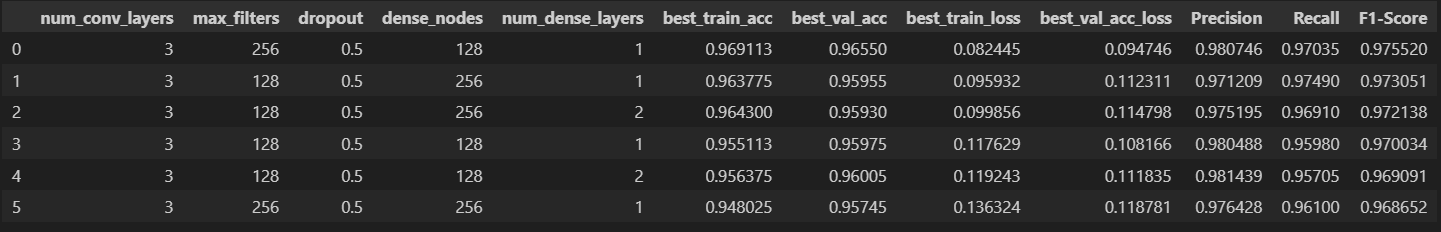
\includegraphics[width=0.8\textwidth]{images/VGG16_hyperparameter.png}
    \caption{Table including all six hyperparameter combinations utilising \texttt{VGG16} as a basemodel.}
    \label{fig:hyperparameters_2}
\end{figure}

The first thing to be noted here is that the accuracy is visibly higher than before, with the best model reaching an accuracy of almost $97 \%$.
This time, we also included the F1-score and recall in our evaluation, hoping to spot possible problems concerning stability earlier.
Further, the issue of instability was also resolved, as can be seen in \autoref{fig:VGG16_hyperparameter_optimisation}.

\begin{figure}[H]
    \centering
    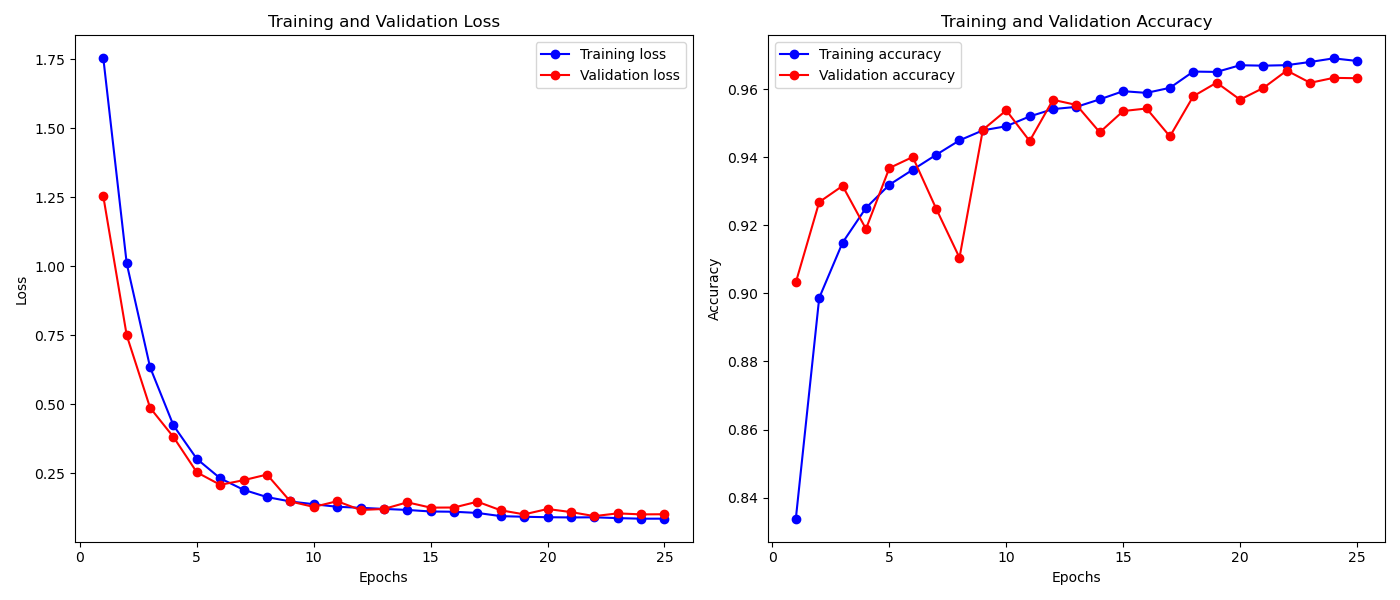
\includegraphics[width=\textwidth]{images/VGG16_best_parameters.png}
    \caption{The $6$ best combinations of hyperparameters for the second approach.}
    \label{fig:VGG16_hyperparameter_optimisation}
\end{figure}

While at the beginning, there still is a slight instability, the validation accuracy now nicely converges against the training accuracy. 

